Die Maxwell-Boltzmann-Verteilung (FoTaBe S.~171) gibt den Bruchteil der Moleküle mit Geschwindigkeiten zwischen $v$ und $v+\mathrm{d}v$ an:
\begin{align}
 \frac{\mathrm{d}N}{N} &= f(v)\,\mathrm{d}v, & f(v) &= 4\pi v^2\left(\frac{m}{2\pi kT}\right)^{3/2}\mathrm{e}^{-\frac{mv^2}{2kT}}
\end{align}
mit der Masse eines Wasserstoffmoleküls $m = M/N_\text{A}$, $M = \MHyF = 2\cdot\MHaO$ (FoTaBe S.~228).

\begin{center}
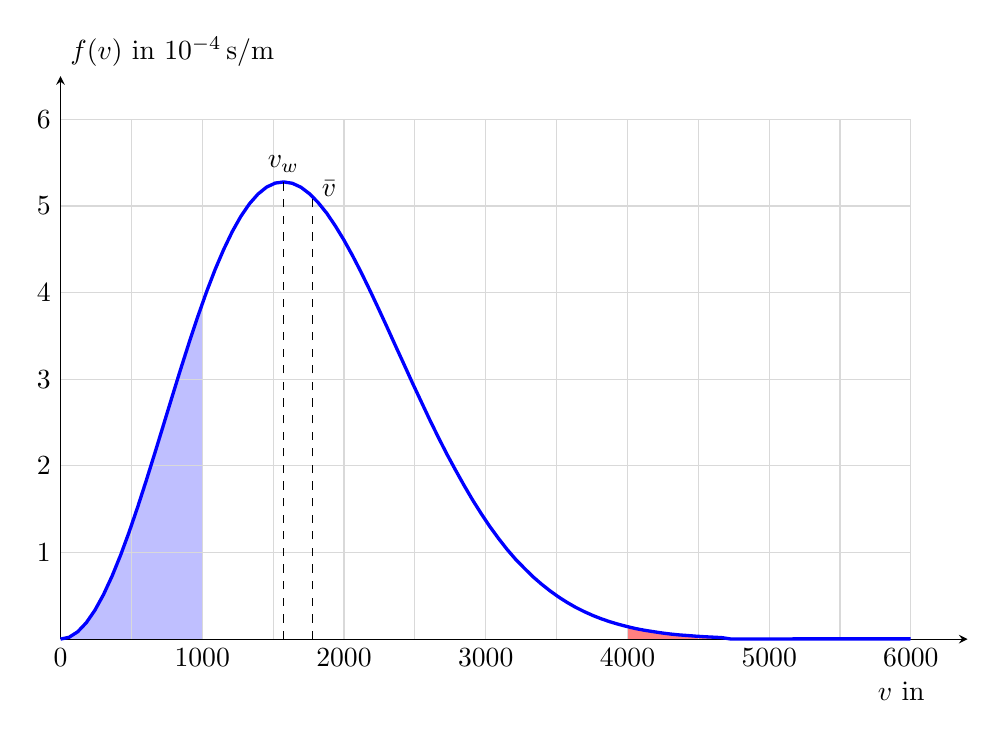
\begin{tikzpicture}[>=stealth, xscale=1.8, yscale=1.1]
 \fill[blue!25, domain=0:1, samples=30] (0,0) -- plot (\x, {5.7984*\x*\x*exp(-((\x/1.573)^2))}) -- (1,0) -- cycle;
 \fill[red!50, domain=4:6, samples=30] (4,0) -- plot (\x, {5.7984*\x*\x*exp(-((\x/1.573)^2))}) -- (6,0) -- cycle;
 \draw[gray!30, xstep=0.5, ystep=1] (0,0) grid (6,6);
 \draw[->] (0,0) -- (6.4,0) node[below left=12pt] {$v$ in \si{\meter\per\second}};
 \draw[->] (0,0) -- (0,6.5) node[above right] {$f(v)$ in $10^{-4}\,\mathrm{s/m}$};
 \foreach \x/\l in {0/0,1/1000,2/2000,3/3000,4/4000,5/5000,6/6000} \node[below] at (\x,0) {\l};
 \foreach \y in {1,2,3,4,5,6} \node[left] at (0,\y) {\y};
 \draw[very thick, blue, domain=0:6, samples=100] plot (\x, {5.7984*\x*\x*exp(-((\x/1.573)^2))});
 \draw[dashed] (1.573,0) -- (1.573,5.28) node[above] {$v_\text{w}$};
 \draw[dashed] (1.775,0) -- (1.775,5.11);
 \node[above right] at (1.775,5.0) {$\bar v$};
\end{tikzpicture}
\end{center}

\begin{abcliste}
\abc Das Maximum liegt bei der wahrscheinlichsten Geschwindigkeit
\begin{align}
 v_\text{w} &= \vwHF = \sqrt{\frac{2\cdot\ncR\cdot\TH}{\MHy}} = \vwH \approx \result{\vwHP{0}{2}}
\end{align}
Die mittlere Schnelligkeit ist grösser,
\begin{align}
 \bar v &= \vmHF = \sqrt{\frac{8\cdot\ncR\cdot\TH}{\pi\cdot\MHy}} = \vmH \approx \result{\vmHP{0}{2}}
\end{align}
also $\bar v/v_\text{w} = \vq$, weil die Verteilung nicht symmetrisch ist: Sie fällt zu hohen Geschwindigkeiten hin langsamer ab, und die schnellen Moleküle heben den Mittelwert an.

\abc Der Bruchteil ist die Fläche unter der Kurve links von \vgAO\ (blau). Numerisches Integrieren mit dem Taschenrechner (oder Auszählen der Gitterfelder) ergibt
\begin{align}
 \frac{\Delta N}{N}\left(v < \vgAO\right) &\approx \result{\anBrP{0}{2}}
\end{align}

\abc Ebenso ist die Fläche rechts von \vgBO\ (rot)
\begin{align}
 \frac{\Delta N}{N}\left(v > \vgBO\right) &\approx \result{\anCrP{0}{2}}
\end{align}

\abc Sauerstoffmoleküle sind sechzehnmal schwerer und deshalb viermal langsamer: Bei \THO\ ist für $\mathrm{O_2}$ $v_\text{w} = \vwOF = \vwOP{0}{2}$ (mit $M = \MOzF$). Weniger als \vgAO\ haben $\anDrP{0}{3}$ der Sauerstoffmoleküle, schneller als \vgBO\ sind praktisch keine.

Ein Teil der Wasserstoffmoleküle ist also sehr schnell. In der obersten Atmosphäre, wo die Temperatur noch viel höher ist und kaum Zusammenstösse stattfinden, erreichen immer wieder Wasserstoffmoleküle (und Heliumatome) die Fluchtgeschwindigkeit der Erde, $v_\text{F} = \vFlO$ (FoTaBe S.~209), und entweichen ins All. Für die schweren Sauerstoff- und Stickstoffmoleküle ist dieser Anteil verschwindend klein. Deshalb ist der leichte Wasserstoff im Lauf der Erdgeschichte fast vollständig aus der Atmosphäre verschwunden, während Stickstoff und Sauerstoff zurückgehalten werden.
\end{abcliste}
